\documentclass[preprint,12pt,aps,pra,showkeys,amsmath,amssymb,superscriptaddress,floatfix]{revtex4-2}
\usepackage[T1]{fontenc}
\usepackage[utf8]{inputenc}
\usepackage{amsmath,amssymb,amsthm,mathtools,mathrsfs}
\usepackage{microtype,booktabs,enumitem}
\usepackage{xcolor,tikz,etoolbox}
\usepackage[skins,breakable]{tcolorbox}
\usepackage{needspace}
% Keep diagram geometry independent of REVTeX preprint body spacing.
\AtBeginEnvironment{tikzpicture}{\linespread{1}\selectfont}
\usetikzlibrary{arrows.meta,positioning,calc,fit,decorations.pathreplacing}
\usepackage{graphicx}
\usepackage{hyperref}

\definecolor{MMBlue}{RGB}{0,82,155}
\definecolor{MMOrange}{RGB}{200,80,0}
\tikzset{
 mmnode/.style={draw=MMBlue,rounded corners=2pt,fill=MMBlue!4,align=left,execute at begin node={\raggedright},text width=5cm,font=\fontsize{10}{12}\selectfont,inner sep=6pt},
 mmimport/.style={mmnode,draw=black!65,fill=black!4},
 mmcandidate/.style={mmnode,draw=MMOrange,dashed,fill=MMOrange!5},
 mmrejected/.style={mmnode,draw=black,densely dotted,fill=black!8},
 mmproof/.style={->,thick,MMBlue},
 mmflow/.style={->,semithick,black!70},
 mmrepair/.style={->,dashed,thick,MMOrange},
 mmcandidatearrow/.style={->,dashed,semithick,MMOrange},
 mmnote/.style={font=\scriptsize,fill=white,inner sep=2pt,align=center}}

\usepackage[section]{placeins}
\setlength{\emergencystretch}{3em}
\setlist{itemsep=3pt,topsep=4pt}
\newtheorem{theorem}{Theorem}[section]
\newtheorem{proposition}[theorem]{Proposition}
\newtheorem{lemma}[theorem]{Lemma}
\newtheorem{corollary}[theorem]{Corollary}
\theoremstyle{definition}
\newtheorem{definition}[theorem]{Definition}
\newtheorem{example}[theorem]{Example}
\theoremstyle{remark}
\newtheorem{remark}[theorem]{Remark}
% Avoid isolated statement headings and single-line paragraph fragments.
\BeforeBeginEnvironment{theorem}{\Needspace{6\baselineskip}}
\BeforeBeginEnvironment{definition}{\Needspace{5\baselineskip}}
\BeforeBeginEnvironment{proposition}{\Needspace{5\baselineskip}}
\BeforeBeginEnvironment{lemma}{\Needspace{5\baselineskip}}
\BeforeBeginEnvironment{corollary}{\Needspace{5\baselineskip}}
\clubpenalty=5000
\widowpenalty=5000
\newcommand{\R}{\mathbb R}\newcommand{\Z}{\mathbb Z}\newcommand{\N}{\mathbb N}
\newcommand{\Pa}{\operatorname{Pa}}\newcommand{\Desc}{\operatorname{Desc}}
\newcommand{\cl}{\operatorname{cl}}\newcommand{\cost}{\operatorname{cost}}
\newcommand{\status}{\operatorname{status}}
% Faculty cards: a visual rail groups the five faculties within one agent.
% The rail has no arrowhead and does not represent a proof dependency.
\newcommand{\mmfacultybadge}[1]{%
 \node[circle,draw=MMBlue,line width=1pt,fill=white,
 minimum size=7mm,inner sep=0pt,font=\sffamily\small\bfseries,text=MMBlue]
 at ([xshift=15pt,yshift=-15pt]frame.north west) {#1};}
\newcommand{\mmfacultyrail}{%
 \draw[MMBlue!80,line width=1pt]
 ([xshift=15pt,yshift=2pt]frame.north west)--
 ([xshift=15pt,yshift=-2pt]frame.south west);}
\newtcolorbox{mmfacultybox}[2]{enhanced,breakable,
 colback=MMBlue!4,colframe=MMBlue!4,boxrule=0pt,arc=3pt,
 left=39pt,right=9pt,top=4pt,bottom=4pt,
 before skip=2pt,after skip=2pt,
 fontupper=\small\linespread{1.1}\selectfont,
 overlay unbroken={\mmfacultyrail\mmfacultybadge{#1}},
 overlay first={\mmfacultyrail\mmfacultybadge{#1}},
 overlay middle={\mmfacultyrail},overlay last={\mmfacultyrail}}
\newcommand{\mmfaculty}[3]{%
 \begin{mmfacultybox}{#1}{#2}
 {\sffamily\bfseries\color{MMBlue}#2}\par\smallskip #3
 \end{mmfacultybox}}
\newcommand{\agent}[9]{%
 \Needspace{8\baselineskip}
 \subsubsection{#1}
 \noindent\textbf{Object.} #2\par
 \noindent\textbf{Role.} #3\par\smallskip
 \mmfaculty{E}{Ego}{#4}
 \mmfaculty{M}{Memory}{#5}
 \mmfaculty{I}{Intellect}{#6}
 \mmfaculty{S}{Sense}{#7}
 \mmfaculty{A}{Action}{#8}
 \smallskip\noindent #9\par}

\usepackage{longtable,array,calc}
\providecommand{\tightlist}{\setlength{\itemsep}{2pt}\setlength{\parskip}{0pt}}
\makeatletter
\def\frontmatter@abstract@produce{\par\addvspace{\frontmatter@preabstractspace}%
\begingroup\prep@absbox\unvbox\absbox\post@absbox\endgroup
\addvspace{\frontmatter@postabstractspace}}
\makeatother
\newcommand{\field}[2]{\par\smallskip\noindent\textbf{#1.} #2\par}
\setlength{\emergencystretch}{5em}
\AtBeginEnvironment{verbatim}{\small\linespread{1.0}\selectfont}


\hypersetup{colorlinks=true,linkcolor=MMBlue,urlcolor=MMBlue,pdfauthor={Dibakar Sigdel}}

\begin{document}

\title{Abel--Ruffini Theorem via an Explicit Quintic\\[4pt]\large An End-to-End Meta-Math Walkthrough}

\author{Dibakar Sigdel}

\affiliation{Mindverse Computing LLC, Lynnwood, WA 98087, USA}

\date{October 2026}

\begin{abstract}

A complete authored walkthrough of abel--ruffini theorem via an explicit
quintic, with explicit mathematical contracts, local verification gates,
and reusable exports. The report presents the target theorem, declared
imports, a dependency graph, five-faculty node contracts, a continuous
proof, a worked example, and a hypothesis-repair audit. It is an
authored mathematical exposition, not a deployed-agent transcript or a
formal proof-assistant certificate.

\end{abstract}\maketitle\linespread{1.12}\selectfont

\noindent\textbf{MA-05 / Modern Algebra / Report v1}

\section{Target and import contract}

\begin{theorem}

Prove \(f(x)=x^5-4x+2\in\mathbb Q[x]\) has Galois group \(S_5\) and is
not solvable by radicals. Deduce there is no radical formula solving
every quintic.

\end{theorem}

\subsection{Foundations and permitted imports}

Use Eisenstein's criterion: a primitive integer polynomial with all
nonleading coefficients divisible by a prime \(\ell\), leading
coefficient not divisible by \(\ell\), and constant coefficient not
divisible by \(\ell ^{2}\) is irreducible over Q. Import
characteristic-zero splitting-field Galois theory, transitivity for
irreducible polynomials, orbit--stabilizer, Cauchy's group theorem,
Lagrange's theorem, and the radical-solvability criterion: a polynomial
over Q is solvable by radicals iff its splitting-field Galois group is
solvable. The permutation generation and \(S_{5}\) nonsolvability steps
are established below.

\clearpage\section{Node interaction workflow}

\begin{center}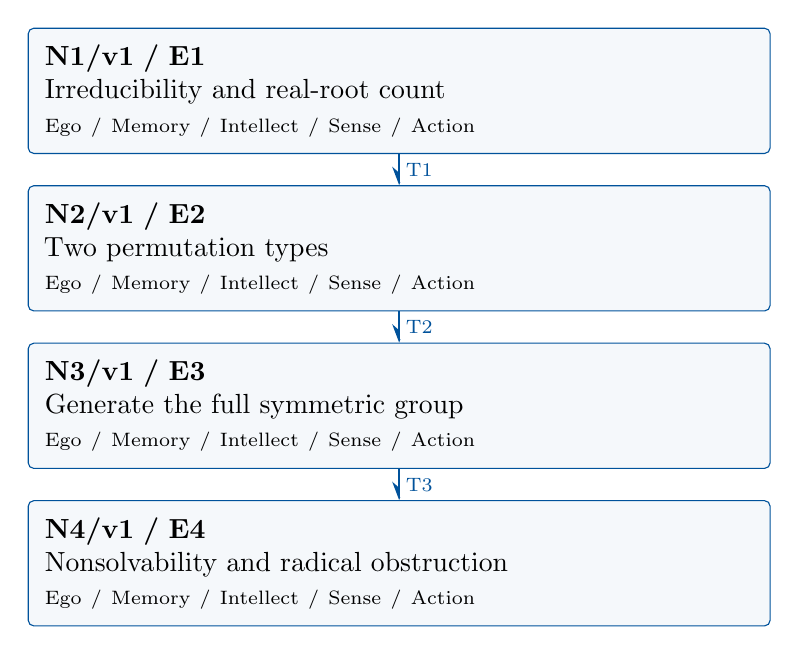
\begin{tikzpicture}[>=Stealth,x=1cm,y=1cm]

\node[mmnode,text width=9cm,minimum height=1.25cm] (N1) at (0,0.0) {\textbf{N1/v1 / E1}\\Irreducibility and real-root count\\{\scriptsize Ego / Memory / Intellect / Sense / Action}};

\node[mmnode,text width=9cm,minimum height=1.25cm] (N2) at (0,-2.0) {\textbf{N2/v1 / E2}\\Two permutation types\\{\scriptsize Ego / Memory / Intellect / Sense / Action}};

\node[mmnode,text width=9cm,minimum height=1.25cm] (N3) at (0,-4.0) {\textbf{N3/v1 / E3}\\Generate the full symmetric group\\{\scriptsize Ego / Memory / Intellect / Sense / Action}};

\node[mmnode,text width=9cm,minimum height=1.25cm] (N4) at (0,-6.0) {\textbf{N4/v1 / E4}\\Nonsolvability and radical obstruction\\{\scriptsize Ego / Memory / Intellect / Sense / Action}};

\draw[mmproof] (N1.south) -- node[mmnote,right] {T1} (N2.north);

\draw[mmproof] (N2.south) -- node[mmnote,right] {T2} (N3.north);

\draw[mmproof] (N3.south) -- node[mmnote,right] {T3} (N4.north);

\end{tikzpicture}\end{center}

Each box is one mathematical agent containing all five faculties. Blue
arrows carry the versioned exports listed below. The layout gives a
reading order; only drawn arrows assert dependencies. Diagnostic repair
is separate from the proof DAG.

\clearpage\subsection{Versioned evidence-transfer ledger}

\begingroup\small\linespread{1.05}\selectfont

\Needspace{5\baselineskip}\field{T1: N1/E1/v1 to N2}{An irreducible quintic with three real roots and one conjugate pair.}

\field{Receiving activity}{N2: Two permutation types}

\field{Compatibility}{Use the same mathematical objects and hypotheses as the source export.
Receiving contract: Irreducibility and real-root count; prior exports
E1/v1}

\Needspace{5\baselineskip}\field{T2: N2/E2/v1 to N3}{G contains a5-cycle and a transposition.}

\field{Receiving activity}{N3: Generate the full symmetric group}

\field{Compatibility}{Use the same mathematical objects and hypotheses as the source export.
Receiving contract: A5-cycle \(\sigma\) and transposition \(\tau\) in G;
prior exports E2/v1}

\Needspace{5\baselineskip}\field{T3: N3/E3/v1 to N4}{The exact Galois group is \(S_{5}\).}

\field{Receiving activity}{N4: Nonsolvability and radical obstruction}

\field{Compatibility}{Use the same mathematical objects and hypotheses as the source export.
Receiving contract: \(G=S_{5}\); radical criterion; prior exports E3/v1}

\endgroup

\clearpage\section{Agent roles and five-faculty activities}\begingroup\small\linespread{1.05}\selectfont\setlist{itemsep=1pt,topsep=2pt}

\subsection{N1/v1: Irreducibility and real-root count}

\field{Object and role}{Combine Eisenstein with exact critical-point signs.}

\field{Inputs}{\(f=x^{5}-4x+2\); foundational imports stated in §1}

\mmfaculty{E}{Ego}{Own E1/v1: An irreducible quintic with three real roots and one
conjugate pair.}

\mmfaculty{M}{Memory}{Retain \(f=x^{5}-4x+2\); foundational imports stated in §1; keep their
assumptions and versions attached.}

\mmfaculty{I}{Intellect}{Combine Eisenstein with exact critical-point signs.}

\mmfaculty{S}{Sense}{A plotted root count alone is not an exact certificate.}

\mmfaculty{A}{Action}{Carry out the numbered deductions and publish E1/v1 together with its
hypotheses and proof location.}

\smallskip\noindent\textbf{Numbered mathematical activities}

\begin{enumerate}[label=N1.\arabic*,leftmargin=3.4em]

\item Eisenstein at 2 applies: the coefficients \(0,0,0,-4,2\) are divisible
by 2 and the constant 2 is not divisible by 4.

\item Thusf is irreducible.

\item Its derivative \(5x^{4}-4\) vanishes at \(\pm \alpha\) where
\(\alpha =(4/5)^{1/4}\); it is positive outside and negative inside.

\item Since \(\alpha >5/8\), \(f(\alpha )=2-(16/5)\alpha <0\) and
\(f(-\alpha )=2+(16/5)\alpha >0\).

\item The limits at \(-\infty\) and \(\infty\) are \(-\infty\) and \(\infty\).

\item Strict monotonicity on the three intervals therefore gives exactly three
distinct real roots and two nonreal roots forming one conjugate pair.

\item Irreducibility over Q in characteristic zero supplies separability, so
all five complex roots are distinct.

\end{enumerate}

\field{Export E1/v1}{An irreducible quintic with three real roots and one conjugate pair.}

\field{Acceptance gate}{A plotted root count alone is not an exact certificate. Publish only
after checking every displayed deduction.}

\field{Targeted repair}{If the check fails, revise N1: A plotted root count alone is not an
exact certificate. Recheck dependent nodes N2, N3, N4.}

\clearpage

\subsection{N2/v1: Two permutation types}

\field{Object and role}{Read transitivity and complex conjugation.}

\field{Inputs}{Irreducibility and real-root count; prior exports E1/v1}

\mmfaculty{E}{Ego}{Own E2/v1: G contains a5-cycle and a transposition.}

\mmfaculty{M}{Memory}{Retain Irreducibility and real-root count; prior exports E1/v1; keep
their assumptions and versions attached.}

\mmfaculty{I}{Intellect}{Read transitivity and complex conjugation.}

\mmfaculty{S}{Sense}{A nonreal-root pair count determines the entire conjugation permutation.}

\mmfaculty{A}{Action}{Carry out the numbered deductions and publish E2/v1 together with its
hypotheses and proof location.}

\smallskip\noindent\textbf{Numbered mathematical activities}

\begin{enumerate}[label=N2.\arabic*,leftmargin=3.4em]

\item Let G be the splitting-field Galois group acting faithfully on five
roots.

\item Irreducibility gives a transitive action, so 5
divides\textbar G\textbar{} by orbit--stabilizer.

\item Cauchy supplies an element of order 5, necessarily a5-cycle in
\(S_{5}\).

\item Complex conjugation is an automorphism of the splitting field fixing Q;
it fixes the three real roots and swaps the nonreal pair, hence is a
transposition.

\end{enumerate}

\field{Export E2/v1}{G contains a5-cycle and a transposition.}

\field{Acceptance gate}{A nonreal-root pair count determines the entire conjugation permutation.
Publish only after checking every displayed deduction.}

\field{Targeted repair}{If the check fails, revise N2: A nonreal-root pair count determines the
entire conjugation permutation. Recheck dependent nodes N3, N4.}

\clearpage

\subsection{N3/v1: Generate the full symmetric group}

\field{Object and role}{Use conjugate transpositions as edges in a connected graph.}

\field{Inputs}{A5-cycle \(\sigma\) and transposition \(\tau\) in G; prior exports E2/v1}

\mmfaculty{E}{Ego}{Own E3/v1: The exact Galois group is \(S_{5}\).}

\mmfaculty{M}{Memory}{Retain A5-cycle \(\sigma\) and transposition \(\tau\) in G; prior
exports E2/v1; keep their assumptions and versions attached.}

\mmfaculty{I}{Intellect}{Use conjugate transpositions as edges in a connected graph.}

\mmfaculty{S}{Sense}{A cycle/transposition claim needs the connected-graph proof; it is not
automatic for arbitrary cycle lengths.}

\mmfaculty{A}{Action}{Carry out the numbered deductions and publish E3/v1 together with its
hypotheses and proof location.}

\smallskip\noindent\textbf{Numbered mathematical activities}

\begin{enumerate}[label=N3.\arabic*,leftmargin=3.4em]

\item Label the roots cyclically so \(\sigma\) acts by addition1 modulo 5, and
write \(\tau =(a,b)\) with nonzero differenceb \(-a\) mod 5.

\item Its conjugates \(\sigma ^j\tau \sigma ^{(-j)}\) swap the translated pair
\(s(a+j,b+j)\).

\item These edges form a connected graph since repeated addition of a nonzero
residue visits all five vertices.

\item Edge transpositions on a connected graph generate every transposition:
along a path, conjugating the final edge swap by the preceding path
swaps gives a swap between the endpoints.

\item All transpositions generateS \(_{5}\), so
\(S_{5}\subset G\subset S_{5}\) and \(G=S_{5}\).

\end{enumerate}

\field{Export E3/v1}{The exact Galois group is \(S_{5}\).}

\field{Acceptance gate}{A cycle/transposition claim needs the connected-graph proof; it is not
automatic for arbitrary cycle lengths. Publish only after checking every
displayed deduction.}

\field{Targeted repair}{If the check fails, revise N3: A cycle/transposition claim needs the
connected-graph proof; it is not automatic for arbitrary cycle lengths.
Recheck dependent nodes N4.}

\clearpage

\subsection{N4/v1: Nonsolvability and radical obstruction}

\field{Object and role}{Prove the needed group obstruction before applying the field theorem.}

\field{Inputs}{\(G=S_{5}\); radical criterion; prior exports E3/v1}

\mmfaculty{E}{Ego}{Own E4/v1: This explicit quintic is not solvable by radicals; no radical
formula covers every quintic.}

\mmfaculty{M}{Memory}{Retain \(G=S_{5}\); radical criterion; prior exports E3/v1; keep their
assumptions and versions attached.}

\mmfaculty{I}{Intellect}{Prove the needed group obstruction before applying the field theorem.}

\mmfaculty{S}{Sense}{Some quintics are solvable; the conclusion is not a claim about every
individual quintic.}

\mmfaculty{A}{Action}{Carry out the numbered deductions and publish E4/v1 together with its
hypotheses and proof location.}

\smallskip\noindent\textbf{Numbered mathematical activities}

\begin{enumerate}[label=N4.\arabic*,leftmargin=3.4em]

\item In \(A_{5}\) the conjugacy-class sizes are 1,15 (double
transpositions),20 (3-cycles), and 12,12 (the two classes of 5-cycles).

\item They follow from cycle counting and centralizer sizes4,3,5 in \(A_{5}\).

\item A normal subgroup is a union of these classes containing the identity,
and its order divides60.

\item The possible such sums are 1,13,25,16,28,40,21,33,45,36,48,60; only1 and
60 divide60.

\item Thus \(A_{5}\) is simple.

\item It is nonabelian, so its nontrivial commutator subgroup, being normal,
is all \(A_{5}\); its derived series never reaches1.

\item Hence \(A_{5}\), and therefore \(S_{5}\) which contains it, is not
solvable.

\item By the imported radical criterion the quintic is not solvable by
radicals.

\item A radical formula for every quintic would solve this one, contradiction.

\end{enumerate}

\field{Export E4/v1}{This explicit quintic is not solvable by radicals; no radical formula
covers every quintic.}

\field{Acceptance gate}{Some quintics are solvable; the conclusion is not a claim about every
individual quintic. Publish only after checking every displayed
deduction.}

\field{Targeted repair}{If the check fails, revise N4: Some quintics are solvable; the
conclusion is not a claim about every individual quintic. Withhold this
terminal result until its gate passes.}

\endgroup\clearpage\section{Continuous mathematical proof}\label{sec:proof}

Read these steps in order as one proof; the diagram is optional.
Numbered activities identify the specific constructions and deductions
owned by each node.

\subsection{§4.N1 --- Irreducibility and real-root
count}\label{n1-irreducibility-and-real-root-count}

\begin{enumerate}
\def\labelenumi{\arabic{enumi}.}
\item
  Eisenstein at 2 applies: the coefficients \(0,0,0,-4,2\) are divisible
  by 2 and the constant 2 is not divisible by 4.
\item
  Thusf is irreducible.
\item
  Its derivative \(5x^{4}-4\) vanishes at \(\pm \alpha\) where
  \(\alpha =(4/5)^{1/4}\); it is positive outside and negative inside.
\item
  Since \(\alpha >5/8\), \(f(\alpha )=2-(16/5)\alpha <0\) and
  \(f(-\alpha )=2+(16/5)\alpha >0\).
\item
  The limits at \(-\infty\) and \(\infty\) are \(-\infty\) and
  \(\infty\).
\item
  Strict monotonicity on the three intervals therefore gives exactly
  three distinct real roots and two nonreal roots forming one conjugate
  pair.
\item
  Irreducibility over Q in characteristic zero supplies separability, so
  all five complex roots are distinct.
\end{enumerate}

\subsection{§4.N2 --- Two permutation
types}\label{n2-two-permutation-types}

\begin{enumerate}
\def\labelenumi{\arabic{enumi}.}
\item
  Let G be the splitting-field Galois group acting faithfully on five
  roots.
\item
  Irreducibility gives a transitive action, so 5
  divides\textbar G\textbar{} by orbit--stabilizer.
\item
  Cauchy supplies an element of order 5, necessarily a5-cycle in
  \(S_{5}\).
\item
  Complex conjugation is an automorphism of the splitting field fixing
  Q; it fixes the three real roots and swaps the nonreal pair, hence is
  a transposition.
\end{enumerate}

\subsection{§4.N3 --- Generate the full symmetric
group}\label{n3-generate-the-full-symmetric-group}

\begin{enumerate}
\def\labelenumi{\arabic{enumi}.}
\item
  Label the roots cyclically so \(\sigma\) acts by addition1 modulo 5,
  and write \(\tau =(a,b)\) with nonzero differenceb \(-a\) mod 5.
\item
  Its conjugates \(\sigma ^j\tau \sigma ^{(-j)}\) swap the translated
  pair \(s(a+j,b+j)\).
\item
  These edges form a connected graph since repeated addition of a
  nonzero residue visits all five vertices.
\item
  Edge transpositions on a connected graph generate every transposition:
  along a path, conjugating the final edge swap by the preceding path
  swaps gives a swap between the endpoints.
\item
  All transpositions generateS \(_{5}\), so
  \(S_{5}\subset G\subset S_{5}\) and \(G=S_{5}\).
\end{enumerate}

\subsection{§4.N4 --- Nonsolvability and radical
obstruction}\label{n4-nonsolvability-and-radical-obstruction}

\begin{enumerate}
\def\labelenumi{\arabic{enumi}.}
\item
  In \(A_{5}\) the conjugacy-class sizes are 1,15 (double
  transpositions),20 (3-cycles), and 12,12 (the two classes of
  5-cycles).
\item
  They follow from cycle counting and centralizer sizes4,3,5 in
  \(A_{5}\).
\item
  A normal subgroup is a union of these classes containing the identity,
  and its order divides60.
\item
  The possible such sums are 1,13,25,16,28,40,21,33,45,36,48,60; only1
  and 60 divide60.
\item
  Thus \(A_{5}\) is simple.
\item
  It is nonabelian, so its nontrivial commutator subgroup, being normal,
  is all \(A_{5}\); its derived series never reaches1.
\item
  Hence \(A_{5}\), and therefore \(S_{5}\) which contains it, is not
  solvable.
\item
  By the imported radical criterion the quintic is not solvable by
  radicals.
\item
  A radical formula for every quintic would solve this one,
  contradiction.
\end{enumerate}

\hfill$\square$

\section{Worked orchestration}

The critical-point audit uses \(\alpha \approx 0.9457\) only as an
illustration; the exact inequality \(\alpha >5/8\) proves the signs. By
contrastx \(^{5}-2\) is irreducible but has roots expressed by a fifth
root and roots of unity, so irreducibility alone cannot imply
nonsolvability.

\subsection{Boundary and hypothesis audit}

A candidate exports ``irreducible quintic \(\Longrightarrow G=S_{5}\).''
Sense counters with \(x^{5}-2\) and with smaller transitive groups. The
repaired route retains both the 5-cycle and single transposition, proves
connected generation, and only then invokes the radical obstruction.

\section{Illustrative failure and repair}

The following is an authored diagnostic scenario. Changed assumptions
define a new contract; they do not retroactively prove the original
statement.

\subsection{Failure and correction}
This is an authored teaching trace, not a recorded agent run.

\begin{enumerate}
\def\labelenumi{\arabic{enumi}.}
\tightlist
\item
  \textbf{Ego \(\to\) Memory:} register the §1 theorem, imports, and
  requested exports before beginning the proof.
\item
  \textbf{Intellect \(\to\) Action:} choose the bridges in §3 and carry
  out the numbered activities in §4; transmit only established E-exports
  along the §2 DAG.
\item
  \textbf{Sense \(\to\) responsible node:} test the specific
  boundary/failure in §5 and the node's individual audit. A failing
  candidate is withheld; downstream nodes may not use it.
\item
  \textbf{Memory + Intellect:} identify whether the error is an omitted
  condition, an invalid inference, or an attempted extension beyond the
  theorem. Restore the exact contract or explicitly state a different
  one.
\item
  \textbf{Action:} redo the affected mathematical activity using the
  repaired condition or inference. Recheck consuming nodes, rather than
  feeding their conclusions back as premises.
\item
  \textbf{Ego:} publish only the supported export with its assumptions
  and proof location. A hypothetical revised export is v2; the written
  proof here is the v1 exposition, not a claim that this repair was
  executed.
\end{enumerate}

\subsection{Hypothesis boundary}
A candidate exports ``irreducible quintic \(\Longrightarrow G=S_{5}\).''
Sense counters with \(x^{5}-2\) and with smaller transitive groups. The
repaired route retains both the 5-cycle and single transposition, proves
connected generation, and only then invokes the radical obstruction.

\subsection{Version and recheck}
Treat any changed assumption as a new contract. Recheck the revised
export and all of its descendants. A backward diagnostic never
establishes an earlier theorem. This is an authored teaching trace, not
an execution log.

\par\medskip\begingroup\small\linespread{1.0}\selectfont\noindent\textbf{Provenance.} This authored proof is complete relative to its declared imports. Reuse
each export with its assumptions, proof, and version. The original
Markdown remains available for comparison.
\par\endgroup

\par\smallskip\begingroup\small\linespread{1.0}\selectfont\noindent\textbf{Further reading.} \begin{itemize}
\tightlist
\item
  \href{https://ocw.mit.edu/courses/res-18-012-algebra-ii-student-notes-spring-2022/pages/student-notes/}{MIT
  Algebra II notes: field extensions and Galois theory}.
\end{itemize}\par\endgroup

\end{document}
